\documentclass[a4paper]{article}
\usepackage {changepage}
\usepackage{fancyhdr}

\usepackage {fontspec}
\pagestyle{fancy}
\setromanfont{Lantinghei SC Extralight}
\setmonofont{Courier New}
\XeTeXlinebreaklocale ``zh''
\XeTeXlinebreakskip = 0pt plus 1pt
\textheight = 650pt
\begin{document}
\title{实验报告 Lab 4}
\author{姓名:王钦\quad 学号:13349112}
\date{}
\maketitle

\section*{ 1. ICMP and Ping}
\hangindent=4em \hangafter=-200{
	1. The IP address of my host:\verb| 192.168.41.102|,ip.dst:\verb| 143.89.14.2|\\\\
	{\centering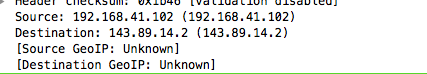
\includegraphics[scale=0.5]{Illustrations/1.png}}\\\\
	2. Because port is in Transport layer,But ICMP is in the ip datagram,So ICMP doesn't have port num.\\\\
	3. IP type:8,code num:0,checksum:0x00006742,icmp.ident:9428,sequence number:4\\\\
	{\centering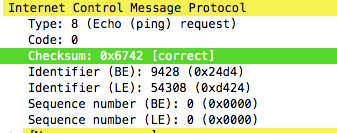
\includegraphics[scale=0.5]{Illustrations/3.png}}\\\\
	4. IP type:0,code num:0,checksum:0x00002efb,icmp.ident:9428,sequence number:4\\\\
	{\centering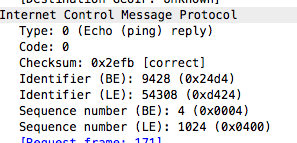
\includegraphics[scale=0.5]{Illustrations/4.png}}\\\\
}
\section*{ 2. ICMP and Traceroute}
\hangindent=4em \hangafter=-200{
	5. The IP address of my host:\verb| 192.168.41.102|,ip.dst:\verb| 128.93.162.84|\\\\
	{\centering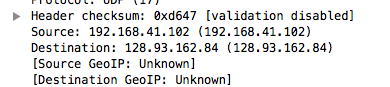
\includegraphics[scale=0.5]{Illustrations/5.png}}\\\\
	6. not 01,Because it above protocol is UDP,so it's protocol number isn't 01 ,instead 0x11.\\\\
	7. The ICMP echo packet has  the same fields as the ping query packets.\\\\	
	8. The ICMP error packet is not the same as the ping query packets.  It contains both the IP header and the first 8 bytes of the original ICMP packet that the error is for.\\\\ 
	{\centering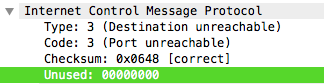
\includegraphics[scale=0.5]{Illustrations/8.png}}\\\\
	9. The last three ICMP packets are message type 0 (echo reply) rather than 11 (TTL expired).  They are different because the datagrams have made it all the way to the destination host before the TTL expired. \\\\
	10. Refer below snapshot between steps 8 and 9 is longer delay.In figure 4 from the lab, There is a link between steps 11 and 12 is longer delay and the link is from New York to Pastourelle, France.\\\\
	{\centering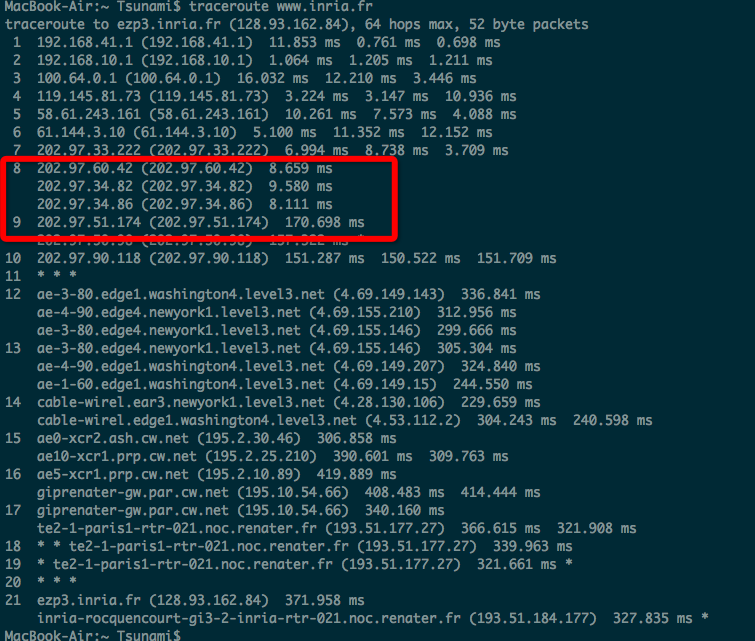
\includegraphics[scale=0.4]{Illustrations/10_1.png}}\\\\
	{\centering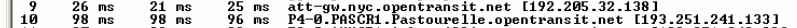
\includegraphics[scale=0.5]{Illustrations/10_2.png}}
}

\section*{ 3. UDP Ping Lab}
\hangindent=4em \hangafter=-200{
  Optional Exercises:\\\\
  \indent I write the Client ,the source file is \verb|PingClient.java|,And the Server source file is \verb|PingServer.java|,all files are in submit Folder.Client can calculate and print RTT of each packet,at last will print the minimum, maximum, and average RTTs.\\\\
  \indent How to use:First open terminal and run command \verb|java PingServer 6000|,mean server will listen \verb|localhost:6000|.
  Second open another terminal run command \verb|java PingClient 6000|,mean client will send ping package to \verb|localhost:6000|,and client run on \verb|localhost:5000|.\\\\
  Client snapshot:\\\\
	{\centering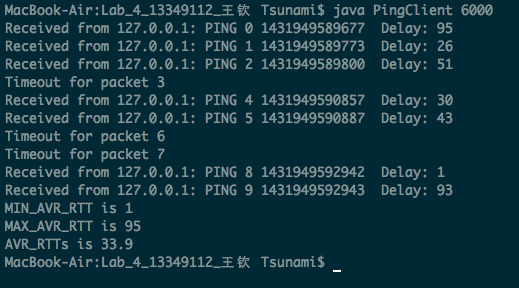
\includegraphics[scale=0.5]{Illustrations/client.png}}\\\\
  Server snapshot:\\\\
	{\centering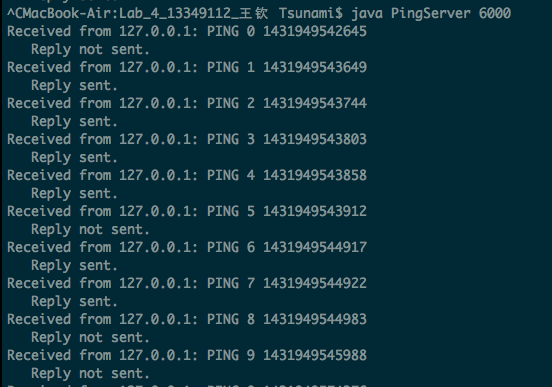
\includegraphics[scale=0.5]{Illustrations/server.png}}\\\\

}

\end{document}

